\begin{slide}
	\begin{block}{Problem}
		Given a $w\cdot{}h$ grid of letters, Find the smallest rectangle which contains at least one \texttt{W},\texttt{A},\texttt{L},\texttt{D} and \texttt{O}.
	\end{block}
	\begin{textblock*}{\paperwidth}(0mm,0.375\paperheight)%
		\only<1>{
		\begin{center}
			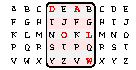
\includegraphics[width=0.5\textwidth]{../problems/lookingforwaldo/problem_statement/sample2.pdf}
		\end{center}}
	\end{textblock*}
	\pause
	\begin{block}{Solution}
		\begin{itemize}
			\item Let $\mathit{next}[x,y,c]$ describe the next occurrence of character $c$ in row $y$ after $x$.
		\end{itemize}
		\begin{overprint}
			\onslide<2>
			\vspace{-\baselineskip}
			\begin{center}
				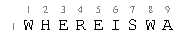
\includegraphics[width=0.5\textwidth]{../problems/lookingforwaldo/solution/sample.pdf}
			\end{center}
			\vspace{-\baselineskip}
			\begin{itemize}
				\item $\mathit{next}[1,1,W]=1$
				\item $\mathit{next}[6,1,W]=8$
				\item $\mathit{next}[9,1,W]=\inf$
			\end{itemize}
			\onslide<3>
			\vspace{-0.5\baselineskip}
			\begin{itemize}
				\item Fix the upper left corner $x, y$ of the rectangle and find the smallest rectangle with height $1,2,\dots$
				\begin{itemize}
					\item For height $1$ this is $\max(\mathit{next}[x,y,c])$ for $c\in{W,A,L,D,O}$.
					\item For height $2$ this is $\max(\min(\mathit{next}[x,y,c], \mathit{next}[x,y+1,c]))$.
					\item For height $h'$, $\min(\mathit{next}[x,y,c],\dots)$ can only decrease to $\mathit{next}[x,y+h'-1,c]$.
					\item[$\Rightarrow$] The inner minimums can be calculated in constant time. The outer maximum can be evaluated in constant time too since it only contains 5 expressions.
				\end{itemize}
			\end{itemize}
		\end{overprint}
	\end{block}
\end{slide}

\begin{slide}
	\begin{block}{Runtime}
		Why is this fast enough?
		\begin{itemize}
			\item There are $w\cdot{}h$ corners we can choose.
			\item The height can be up to $h$
			\item[$\Rightarrow$] The runtime is $\mathcal{O}(w\cdot h\cdot h)$. This sounds quadratic?
			\pause
			\item Note that $n=w\cdot{}h$ was bounded in the input.
			\item If we assume $h\leq w$ the actual runtime is $\mathcal{O}(n\sqrt{n})$ which is fast enough.
			\pause
			\item If $h>w$ we can rotate or transpose the input to make $h\leq w$.
		\end{itemize}
	\end{block}
	\pause
	\begin{block}{Alternatives}
		\begin{itemize}
			\item A faster runtime can be achieved with a \emph{Divide and Conquer} approach, which runs in $\mathcal{O}(n\log{n})$.
			\item However, this was not required.
		\end{itemize}
	\end{block}
\end{slide}
